%%% load packages
\usepackage{geometry}
\usepackage{xcolor}
\usepackage{eso-pic}
\usepackage{atbegshi}
\usepackage{fancyhdr}
\usepackage[explicit]{titlesec}
\usepackage{marginnote}
\usepackage{setspace}
\usepackage{enumitem}
\usepackage[most]{tcolorbox}
\usepackage{graphicx}
\usepackage{tikz}
\usepackage{pagecolor}
\usepackage{anyfontsize}
\usepackage[table, dvipsnames]{xcolor} % KEIN 'html'!
\usepackage{transparent}
\usepackage{tikzpagenodes}
\usepackage{ifthen}




%%% --- Define Colors ---
% Define Colors
\definecolor{my_orange}{HTML}{FF8E00}
\definecolor{blender_blue}{HTML}{236192}
\definecolor{remember_gold}{HTML}{FFDE7E}
\definecolor{orangeTop}{HTML}{FFA600}
\definecolor{orangeBottom}{HTML}{FF8E00}
\definecolor{blue_box}{HTML}{1E6AE2}




%%% --- Adjust Document Settings ---
% Set page size
\geometry{a4paper, inner=30mm, outer=40mm, top=25mm, bottom=25mm}

% Activate fancy-Style
\pagestyle{fancy}

% Delete default-Styles
\fancyhf{}






%%% --- Adjust Font ---
\renewcommand{\normalsize}{\fontsize{10pt}{13pt}\selectfont}
\makeatletter
\renewcommand\normalsize{%
  \@setfontsize\normalsize{12pt}{15pt}% 12pt Schrift und 15pt Zeilenabstand
  \abovedisplayskip 10pt plus 2pt minus 5pt%
  \abovedisplayshortskip \z@ plus 2pt%
  \belowdisplayshortskip 6pt plus 2pt minus 3pt%
  \belowdisplayskip \abovedisplayskip
  \let\@listi\@listI%
}
\makeatother
\normalsize

\makeatletter
\renewcommand\small{\@setfontsize\small{9pt}{11pt}}
\renewcommand\footnotesize{\@setfontsize\footnotesize{8pt}{10pt}}
\makeatother


% Increase space between lines
\setstretch{1.2}

% Remove spacing after lists
\setlist{nosep}

% Remove spacing for new paragraphs
\setlength{\parskip}{0pt}

% Adjust spacing after titles (\Section, left, before, after)
\titlespacing*{\chapter}{0pt}{0pt}{0pt}
\titlespacing*{\section}{0pt}{10pt}{0pt}
\titlespacing*{\subsection}{0pt}{10pt}{0pt}
\titlespacing*{\subsubsection}{0pt}{10pt}{0pt}





%%% --- Adjust Margins ---
% Change marginnotes
\let\oldmarginnote\marginnote

% Define width off the marings
\setlength{\marginparwidth}{3cm}


\renewcommand{\marginnote}[1]{%
  \oldmarginnote{{\footnotesize\selectfont #1}}%
}





%%% --- Adjust chapter titles ---
% Remove "Chapter"-prefix from chapter-title
%Adjust title format
\titleformat{\chapter}[hang]
  % Font of the title
  {\normalfont\huge\bfseries}
  % Suppress Chapter-Number
  {\thechapter.\quad}
  % Remove space after (removed) chapter number
  {0pt}
  % Execute Chapter-title
  {#1}





%%% --- Adjust Page Header ---
% Remove default-Header
\renewcommand{\headrulewidth}{0pt}

% Increase space between header and text
\setlength{\headsep}{30pt}

% Set text for heading
\makeatletter
\renewcommand{\chaptermark}[1]{\markboth{#1}{}}
% Remove "Chapter"-Prefix
\renewcommand{\@chapapp}{}
\makeatother


%%% Odd pages (Recto)
\newcommand{\headerRecto}{%
  \AddToShipoutPictureFG*{%
    \begin{tikzpicture}[remember picture, overlay]
      \fill[my_orange] ([yshift=-30pt]current page.north west) rectangle ([yshift=-60pt]current page.north east);
      \node[anchor=west, text=white, font=\bfseries, yshift=-45pt, xshift=90pt]
        at (current page.north west) {\phantom{00}};
      \node[anchor=east, text=white, font=\bfseries, yshift=-45pt, xshift=-80pt]
        at (current page.north east)  {Creating the World};
    \end{tikzpicture}%
  }
}

%%% Even pages (Verso)
\newcommand{\headerVerso}{%
  \AddToShipoutPictureFG*{%
    \begin{tikzpicture}[remember picture, overlay]
      \fill[my_orange] ([yshift=-30pt]current page.north west) rectangle ([yshift=-60pt]current page.north east);
      \node[anchor=west, text=white, font=\bfseries, yshift=-45pt, xshift=80pt]
        at (current page.north west) {Creating the World};
      \node[anchor=east, text=white, font=\bfseries, yshift=-45pt, xshift=-90pt]
        at (current page.north east) {\phantom{00}};
    \end{tikzpicture}%
  }
}


%% Asign header to odd pages
\fancyhead[LO,RO]{\headerRecto}

%% Asign header to even pages
\fancyhead[LE,RE]{\headerVerso}

%% Asign header to even pages

%% Overwrite plain-Style at beginning of chapter
\fancypagestyle{plain}{%
  % Remove headers
  \fancyhf{}
  % No additional lines
  \renewcommand{\headrulewidth}{0pt}
  %% Asign header to even pages
  \fancyhead[LO,RO]{\headerRecto}
  %% Asign header to odd pages
  \fancyhead[LE,RE]{\headerVerso}
}





%%% --- Define Boxes ---
%## Tipp-box
% Define new colorbox
\newtcolorbox{tipp}[1]{
% Add space before box and cener box
before=\bigskip\centering,
% Add space after the box
after=\bigskip,
% Activate enhanced mode of colorbox
enhanced,
% Create round corners
arc=10pt,
% Create gold frame
colframe=green!75!black,
% Craete gold background color
colback=green!5!white,
% Define Font of title (black font, sans-serife and large)
fonttitle=\sffamily\bfseries\normalsize,
% Set content 1 as title
title=#1,
% Add space before and after the title inside the box
title={\vspace{2.5mm}#1\vspace{2.5mm}},
% Set space in upper left corner 
leftupper=2.5cm,
% Set round corners
rounded corners,
% Fix title to top of box
attach boxed title to top,
frame hidden,
% Define style of title
boxed title style={
    % Activate enhanced settings of title-field
    enhanced,
    % Set frame of title box
    colframe=green!75!black,
    % Set background of title box
    colback=green!75!black,
    % Set round-angle of title field
    arc=10pt,
    % Supress frame around title fileld
    bottomrule=0pt,
    rightrule=0pt,},
  % Overlay image
  overlay={
    % Set anchor north-west
    \node[anchor=north west] 
      % Adjust position in relation to frame
      at ([xshift=10pt,yshift=-1.75\baselineskip]frame.north west)
        % Add image
       {
\includegraphics[width=1cm]{"icons/info.png"}};}}



%%%%% Exercise
% Define new colorbox
\newtcolorbox[auto counter]{exercise}[2][]{
% Add space before box and cener box
before=\bigskip\centering,
% Add space after the box
after=\bigskip,
% Activate enhanced mode of colorbox
enhanced,
% Create round corners
arc=15pt,
% Create blue frame
colframe=blender_blue,
% Craete blue background color
colback=blender_blue!5!white,
% Define Font of title (black font, sans-serife and large
fonttitle=\sffamily\bfseries\Large,
% Set title
title=Übung~\thetcbcounter,
% Define sharp corners
sharp corners,
% Set space in upper left corner 
leftupper=2.5cm,
% Overlay image
overlay={
  % Set anchor north-west
  \node[anchor=north west] 
    % Adjust position
    at ([xshift=10pt,yshift=-.65\baselineskip]frame.north west)
     % Add image
     {\includegraphics[width=1cm,height=1cm]{"icons/exercise.png"}};},
% Set round corners
rounded corners=northeast,
% Fix title to top of box
attach boxed title to top left,
% Define style of title
boxed title style={
    % Activate enhanced settings of title-field
    enhanced,
    % Set frame of title box
    colframe=blender_blue,
    % Set background of title box
    colback=blender_blue,
    % Set round-angle of title field
    arc=5pt,
    % Supress frame around title fileld
    bottomrule=0pt,
    rightrule=0pt,
    % Set sharp corners
    sharp corners,
    % Set round corners norh-east
    rounded corners=northeast,},
% Define stly of (emtpy) interior block
interior style={},
% Define style of frame
frame style={
    % Set colors
    color= cyan!5!white,
    fill=none},
% Align additional overlays
overlay unbroken and first={
    % Place text
    \node[anchor=west,font=\sffamily\bfseries,color=blue] 
    % Position text east of title and with large font
    at (title.east) {{\Large #2}};
    %
    \node[anchor=north west] 
    % Set position
    at ([xshift=10pt, yshift=-1.75\baselineskip]frame.north west)
      % Add image
     {\includegraphics[width=1.5cm]{"icons/exercise.png"}};},#1}



%%%%% Remember
% Define new colorbox
\newtcolorbox{remember}[1]{
% Add space before box and cener box
before=\bigskip\centering,
% Add space after the box
after=\bigskip,
% Activate enhanced mode of colorbox
enhanced,
% Create round corners
arc=10pt,
% Create gold frame
colframe=remember_gold,
% Craete gold background color
colback=remember_gold,
% Define Font of title (black font, sans-serife and large
fonttitle=\color{black}\sffamily\bfseries\Large,
% Set content 1 as title
title=#1,
% Add space before and after the title inside the box
title={\vspace{2.5mm}#1\vspace{2.5mm}},
% Set space in upper left corner 
leftupper=2.5cm,
% Set round corners
rounded corners,
% Fix title to top of box
attach boxed title to top,
% Define style of title
boxed title style={
    % Activate enhanced settings of title-field
    enhanced,
    % Set frame of title box
    colframe=remember_gold,
    % Set background of title box
    colback=remember_gold,
    % Set round-angle of title field
    arc=10pt,
    % Supress frame around title fileld
    bottomrule=0pt,
    rightrule=0pt
    },
  % Overlay image
  overlay={
    % Set anchor north-west
    \node[anchor=north west] 
      % Adjust position in relation to frame
      at ([xshift=10pt,yshift=-1.75\baselineskip]frame.north west)
        % Add image
       {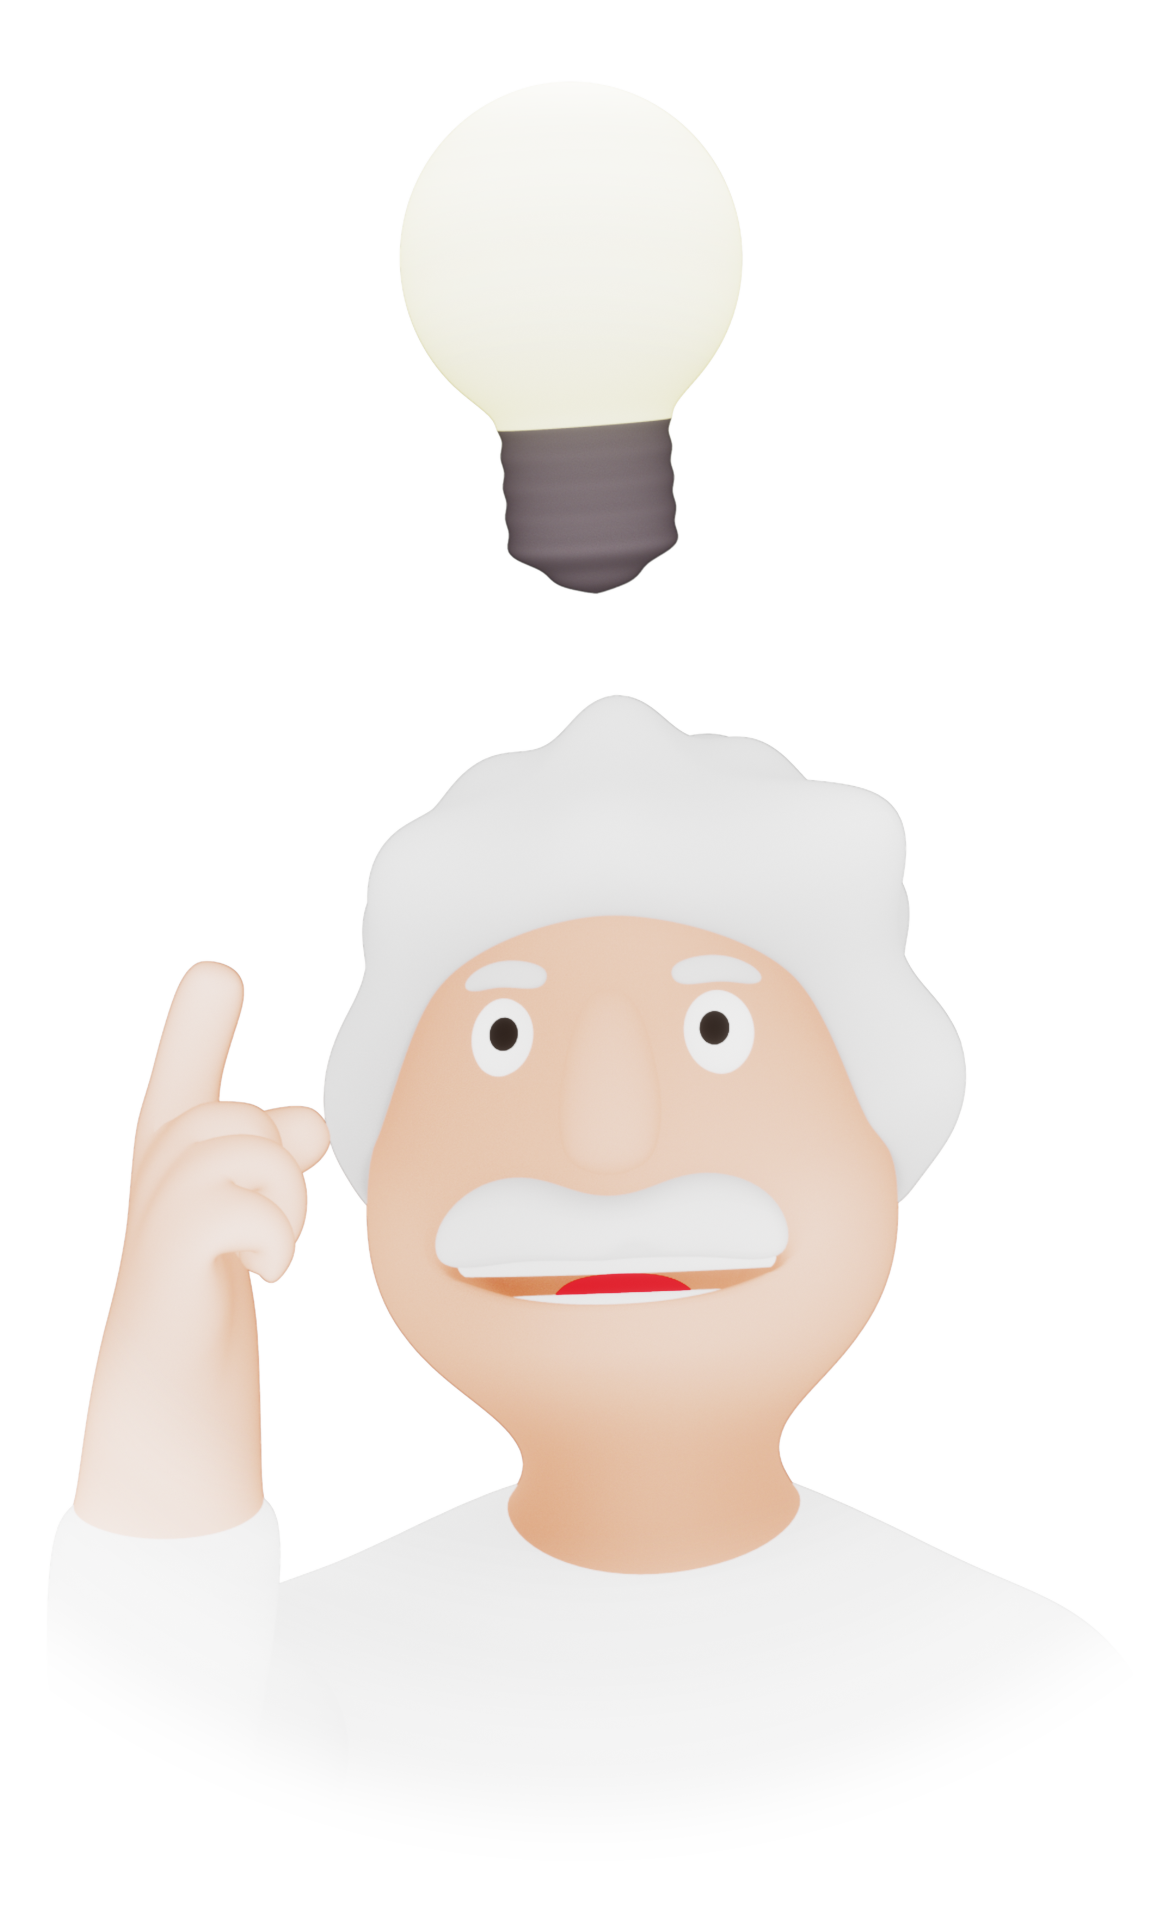
\includegraphics[width=1cm]{"icons/remember.png"}};}}
       


%%%%% Footer
\newcommand{\seitenzahlInFusszeile}{%
  \AddToShipoutPictureFG*{%
    \begin{tikzpicture}[remember picture, overlay]
      \ifodd\value{page}
        % Odd pages - box left
        \node[anchor=south west, font=\normalfont\small, text=black] 
          at ([xshift=29mm, yshift=0.65cm]current page.south west) {\thechapter.\ \leftmark};
        \node[anchor=south east] 
          at ([xshift=-2.0cm]current page.south east) {%
            \raisebox{-0.15\baselineskip}{%
              \colorbox{blue_box}{%
                \parbox[c][1.25\baselineskip][t]{0.5cm}{%
                  \vspace{0.28\baselineskip}%
                  \centering\color{white}\bfseries\small\thepage%
                }%
              }%
            }%
          };
      \else
        % even pages - box right
        \node[anchor=south east, font=\normalfont\small, text=black] 
          at ([xshift=-29mm, yshift=0.65cm]current page.south east) {\thechapter.\ \leftmark};
        \node[anchor=south west] 
          at ([xshift=2.0cm]current page.south west) {%
            \raisebox{-0.15\baselineskip}{%
              \colorbox{blue_box}{%
                \parbox[c][1.25\baselineskip][t]{0.5cm}{%
                  \vspace{0.28\baselineskip}%
                  \centering\color{white}\bfseries\small\thepage%
                }%
              }%
            }%
          };
      \fi
    \end{tikzpicture}%
  }
}


\AtBeginShipout{%
  \ifthenelse{%
    \NOT\(\value{page}=1 \OR \value{page}=2\)%
  }{%
    \seitenzahlInFusszeile%
  }{}%
}